\section{Action Planning and Scheduling}\label{sec:plan}

% Haben Support

% Schon gemacht:
% Meeting IT-Management TUM: Zugriff TumONline
% Meeting Physik: Hardware

%TODO: blabla und Bild kleiner machen!



The Gantt chart in chapter gives a brief overview of all tasks necessary for the proposed project.
It lists important milestones, estimates task lengths and assigns them to the three team members\footnote{In this context, `St' stands for `Stefan', `Se' for `Sebastian' and `Bj' for `Björn'}.

The chart includes tasks since the start of the project.
These already finished steps focused on conceptual and organisational aspects.
Most importantly, we obtained approval of important TUM stakeholders:
\begin{itemize}
\item Mr.~Bernhofer from the TUM IT Management, responsible for identity management and connections to external IT systems. He provided us with information how to access central TUM services (Active Directory, ...).
\item Mr.~Recksiegel from the TUM physics department, who is the head behind an existing student card to NFC solution running in the physics building. He promised help with hardware issues and to finally push the integration of our smartphone to NFC solution into the already existing systems.
\end{itemize}

%Mr.~Recksiegel also mentioned another possible field of application: 
%die Duschen halt....






%\newpage



\par\vfill\break % Break Last Page

\advance\vsize by 6cm % Advance page height
\advance\voffset by -2cm % Shift top margin
% Start big page
\centerline{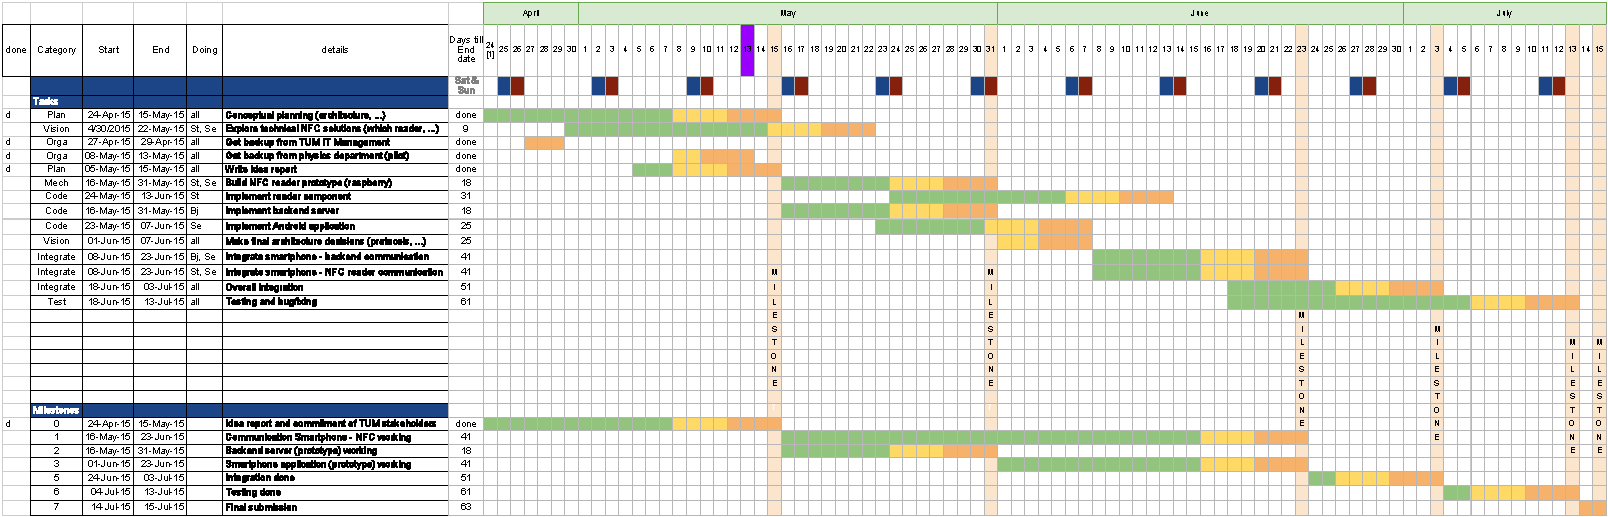
\includegraphics[angle=270]{plan-crop.pdf}}
% End big page
\par\vfill\break % Break the page with different margins

\advance\vsize by -6cm % Return old margings and page height
\advance\voffset by 2cm % Return old margings and page height